\chapter{Схема Неймана-Улама и её обобщение на нелинейные уравнения}
Деревья конструкции, аналогичной описанной в главе \ref{chapter:2}, используются в известном обобщении схемы Неймана-Улама, что приводит к идее применения оценок, разработанных для линейных интегральных уравнений, к задаче нахождения цены Американского опциона. Ниже будут изложены общие сведения о схеме Неймана-Улама и проведены более детальные аналогии с оценками \eqref{eq:common_recursive_statement}.

% Пусть $\mathfrak{X}$ --- локально компактное хаусдорфово пространство, $\mu$ --- $\sigma$-конечная мера Радона на $\mathfrak{X}$. Обозначим пространство вещественных функций, $r$-я степень которых интегрируема относительно меры $\mu$, как $L^r\left(\mathfrak{X}, \mu\right)$ (или просто $L^r$ в тех случаях, когда это не порождает неоднозначность). Объектом интереса будет являться уравнение вида
% \begin{equation} \label{eq:integral}
% 	\vfi = \mathcal{K}\vfi + f,
% \end{equation}
% где $\mathcal{K}: L^r \to L^r$ --- регулярный интегральный оператор с ядром $K: \mathfrak{X}\to \mathfrak{X}$, $f\in L^r$, а $\sum_{i=0}^\infty \mathcal{K}^i f$ сходится по метрике в $L^r$.

% $\forall\,\vfi$ --- решение уравнения \eqref{eq:integral}, $h\in L^t\left(\mathfrak{X}, \mu\right)$ для $t:\nicefrac{1}{t} + \nicefrac{1}{r} = 1$ определено $\left(h, \vfi\right) = \int h\left(x\right)\vfi\left(x\right) d\mu$, причём $\left(h,\vfi\right) = \sum_{i=1}^\infty \left(\mathcal{K}^i f, h\right)$. Следовательно\footnote{Более подробно --- в \cite{montekarlo1975}}, можно представить $\left(\vfi,h\right)$ как
% \begin{equation}
% 	\left(\vfi, h\right) = \sum_{i=1}^\infty \int_{\mathfrak{X}^{i+1}}f(x_0)K(x_0, x_1)\cdots K(x_{i-1}, x_i)h\left(x_i\right)\mu^id\left(x_1,\ldots,x_i\right).
% \end{equation}
% Будем далее обозначать $K\left(x_{i-1}, x_i\right) = K_{i-1, i}, f\left(x_i\right) = f_i, h\left(x_i\right) = h_i$.

% Рассмотрим теперь марковскую цепь с поглощением, определяемую начальным распределением $\pi\left(x\right): \int_{\mathfrak{X}} \pi(x) dx = 1$ и переходной плотностью 
% $$p\left(x_{i-1}, x_i\right) \geq 0 : \:\forall x \int_\mathfrak{X} p(x, x_i)\mu(dx_i) = 1 - g(x) \mod \mu,$$
% $g\in\left[0;1\right)$ $\mu$-почти всюду, $g$ --- вероятность <<поглощения>>, обрыва траектории. Будем далее обозначать аналогично операторам в интегральном уравнении $p\left(x_{i-1}, x_i\right) = p_{i-1, i}, g\left(x_i\right) = g_i, \pi\left(x_i\right) = \pi_i$.

% Для марковской цепи \emph{выполняются условия согласования}, если $\forall \left(x_0, \ldots, x_k\right) \in \mathfrak{X}$
% 	\[
% 		f_0 K_{0,1}\cdots K_{k-1, k} h_k \not = 0 \mod \mu^{k+1} \implies p_0 p_{0,1}\cdots p_{k-1, k} g_k > 0 \mod \mu^{k+1}.
% 	\]
% \newpage
\section{Общие сведения о схеме Неймана-Улама применительно к ветвящемуся марковскому процессу}\label{sec:neyman-ulam}
Пусть имеется уравнение 
\begin{equation}
	\vfi\left(x\right) = \int K\left(x, y, \vfi\left(y\right)\right)\vfi\left(y\right) \mu\left(dy\right) + f\left(x\right) \quad \mod \mu,
\end{equation}
для которого сходится метод последовательных приближений
\begin{equation}
	\vfi_n\left(x\right) = \int K\left(x, y, \vfi_{n-1}\left(y\right)\right)\vfi_{n-1}\left(y\right) \mu\left(dy\right) + f\left(x\right) \quad \mod \mu,
\end{equation}
для некоторого начального приближения $\vfi_0\left(x\right)$ при $n\to\infty$. Тогда при наличии предположений о сходимости ряда Неймана $\sum_{i=0}^\infty \int K^i f d\mu$ в той же метрике, в которой сходится метод последовательных приближений, об устойчивости ядра $K$ интегрального оператора к возмущениям, и, возможно, некоторых других, можно получать приближённые решения $\vfi_n$ методом Монте-Карло.

Процесс отыскания численного решения усложняется тем, что неизвестным в интегральном уравнении является функция, а не число, что означает дополнительные вопросы о способе хранения информации о решении уравнения. Представленный ниже способ, как будет видно, избавляет от необходимости хранить таблицу значений искомой функции.

Будем рассматривать только <<одночленные>> уравнения вида 
\begin{align}
	\vfi\left(x\right) &= \int K\left(x, y_1, \ldots,y_b\right)\prod_{i=1}^b\vfi\left(y_i\right)\mu^b\left(dy_1, \ldots,dy_b\right) + f\left(x\right) \Longleftrightarrow \label{eq:tree-basic}\\
	\Longleftrightarrow \vfi &= \mathcal{K}\vfi^{\left(b\right)} + f \nonumber
\end{align}
и предполагать, что метод последовательных приближений 
\begin{equation}
\label{eq:consecutive-approximations}
\vfi_0 = f, \quad\vfi_n = \mathcal{K}\vfi_{n-1}^{(b)} + f
\end{equation}

сходится в метрике некоторого банахова пространства $F$ к решению уравнения \eqref{eq:tree-basic}.

Рассмотрим пример для $b=2, n=2$.
\begin{align*}
\vfi_1\left(x_0\right) = &f(x_0) + \int K\left(x_0, x_1, x_2\right)f(x_1)f(x_2)\mu^2\left(dx_1,dx_2\right) \\
\vfi_2(x_0) = &f(x_0) + \int K\left(x_0, x_1, x_2\right)\times \\
% \times\left[f(x_1) + \int K\right]\times \\
\times&\left[f(x_1) + \int K\left(x_1, x_3, x_4\right)f(x_3)f(x_4)\mu^2\left(dx_3,dx_4\right)\right]\times \\
\times&\left[
	f(x_2) + \int K\left(x_2, x_5, x_6\right)f(x_5)f(x_6)\mu^2\left(dx_5,dx_6\right)
\right]\times\mu^2\left(dx_1,dx_2\right) =\\
=& f_0 + \int K_{0,1,2}f_1f_2\mu_{1,2} + 
	\int K_{0,1,2}\left(f_1\int K_{2,5,6}f_5f_6\mu_{5,6}\right)\mu_{1,2} + \\
	&+ \int K_{0,1,2}\left(f_2\int K_{1,3,4}f_3f_4\mu_{3,4}\right)\mu_{1,2} + \\
	&+ \int\int\int K_{0,1,2}K_{1,3,4}K_{2,5,6}f_3f_4f_5f_6\mu_{1,2}\mu_{3,4}\mu_{5,6}
\end{align*}
Если посмотреть на дерево вида \ref{fig:exponential_tree}, можно заметить, что переменные в слагаемых вышеприведённого уравнения в точности соответствуют поддеревьям полного дерева, у которого из каждой вершины выходит $b=2$ дочерних, а расстояние от корня до листьев равно $n=2$.

Обозначив последовательности $j_1\cdots j_k$ мультииндексами $\nu[0] = (1), \;\nu[k+1] = (\nu[k], j_{k+1})$, можно выразить уравнение метода последовательных приближений \eqref{eq:consecutive-approximations} как
$$
	\begin{aligned}
		\vfi_{N-k}\left(x\left[\nu(k)\right]\right) = 
		&\int K\left(
			x\left[\nu(k)\right], x\left[\nu(k),1\right], \ldots ,x\left[\nu(k),b\right]
		\right) \times \\
		&\times\prod_{j_{k+1} = 1}^b \vfi_{N-k-1}\left(x\left[\nu(k+1)\right]\right)\mu^b\left(
			dx\left[\nu(k), 1\right],\ldots,dx\left[\nu(k),b\right]
		\right) + \\
		&+ f\left(x\left[\nu(k)\right]\right),
	\end{aligned}
$$
а введя сокращённые обозначения 
$$
	\begin{aligned}
	z\left[\nu\left(k\right)\right] &= \vfi_{N-k}\left(x\left[\nu(k)\right]\right), \\
	a_{\nu\left(k\right)}\vfi &= \int K\left(
			x\left[\nu(k)\right], x\left[\nu(k),1\right], \ldots ,x\left[\nu(k),b\right]
		\right) \vfi d\mu, \\
	f\left[\nu\left(k\right)\right] &= f\left(x\left[\nu(k)\right]\right),
	\end{aligned}
$$
переписать в виде
$$
	z\left[\nu\left(k\right)\right] = a_{\nu\left(k\right)}\prod_{j_{k+1} = 1}^b z\left[\nu\left(k+1\right)\right] + f\left[\nu\left(k\right)\right].
$$

Каждый мультииндекс $\nu(k)$ является описанием некоторой траектории, а в силу конструкции индексов эти траектории сливаются в дерево. Для дальнейшей работы дадим более формальное описание деревьев.

Пусть $\gamma_k = \left(\GothB_0,\ldots,\GothB_k\right)$ --- совокупность множеств $\GothB_r, r\in \mathbb{N}\cup\left\lbrace 0\right\rbrace$ мультииндексов $\nu(r)$, удовлетворяющих следующим условиям:
\begin{enumerate}
	\item $\forall\: r > 1, \:\nu(r)\in \GothB_r$ соответствующее $\nu(r-1)\in\GothB'_{r-1}\subset\GothB_{r-1}$.
	\item $\forall\; r > 0 \:\nu(r) = \left(\nu(r-1), j_r\right)$, и $j_r$ принимает всевозможные значения из $1:b$.
	\item $\GothB_0 = \left\lbrace\left(1\right)\right\rbrace$.
\end{enumerate}
Такую совокупность $\gamma_k$ назовём деревом. Дерево, для которого все $\GothB'_{r-1} = \GothB_{r-1}$, называется полным. Множество $\GothB'_{r}$ здесь по сути является множеством, траектории из которого <<продолжат существование>> на следующем шаге. Так, дерево с рис. \ref{fig:exponential_tree} имеет $\GothB'_1 = \cup_{b=1}^3 \left\lbrace (1, b,1), (1,b,2), (1,b,3)\right\rbrace$ и $\GothB'_2 = \emptyset$. Для любого дерева $\gamma$ определён оператор
\begin{equation}\label{eq:tree-operator}
	\begin{aligned}
	A\left(\gamma\right) = &f\left[\nu(0)\right] \text{ при } N=0 \\
	A\left(\gamma\right) = &a_{\nu(0)}\prod_{\GothB_1\setminus\GothB'_1}f\left[\nu(1)\right]\prod_{\GothB'_1}a_{\nu(1)} \prod_{\GothB_2\setminus\GothB'_2}f\left[\nu(1)\right]\prod_{\GothB'_2}a_{\nu(2)} \times \\
	&\times\cdots\times \prod_{\GothB_N}f\left[\nu(N)\right] \text{ при } N>0
	\end{aligned} 
\end{equation}

% Оператор \ref{eq:tree-operator} определён с некоторыми вольностями в обозначениях: так, для оператора и функции
% 	$$a_{\nu(k)} f\left[\nu\left(k\right)\right] = \int K\left(
% 			x_{\nu(k)}, x_{\nu(k), 1}, \ldots, x_{\nu(k), b}
% 		\right)
% 		\prod_{j=1}^b f\left[\nu(k), j\right]
% 		dx_{\nu(k), 1}, \ldots, dx_{\nu(k), b},$$ тогда как та же запись для двух операторов обозначает их композицию 
% 		\begin{multline}
% 		a_{\nu(k)} a_{\nu(k+1)} = \int K\left(
% 				x_{\nu(k)}, x_{\nu(k), 1}, \ldots, x_{\nu(k), b}
% 			\right) \times \\ \times\prod_{j=1}^b \int K\left(
% 				x_{\nu(k), j}, x_{\nu(k), j, 1}, \ldots, x_{\nu(k), j, b}
% 			\right)\;\bullet\;dx_{\nu(k), j, 1}, \ldots, dx_{\nu(k), j, b} \\
% 			dx_{\nu(k), 1}, \ldots, dx_{\nu(k), b}.
% 		\end{multline}
		
В \cite{montekarlo1975} доказано, что 
\begin{equation}\label{eq:subtrees}
z\left[\nu(0)\right] = \sum_{\gamma\in\Gamma_N}A\left(\gamma\right),
\end{equation}
где суммирование проходит по всем поддеревьям полного дерева с $N$ поколениями $\Gamma_N$.

В результате реализации однородного ветвящегося марковского процесса с начальной плотностью $\pi\left(x\right) \geq 0$, переходной плотностью $p(x,y_1,\ldots,y_b) \geq 0$ и вероятностью поглощения $g\left(x\right): \int p(x,y_1,\ldots,y_b) \mu^s\left(dy_1, \ldots, dy_b\right) = 1 - g(x)$ образуется дерево описанного выше типа, число поколений которого $N$ не обязательно конечно. В случае, если конкретная реализация $\gamma$ имеет длину $N\in(0;\infty)$, то ей соответствует плотность вероятности
\begin{align*}
	p(\gamma) = &\pi\left(x\left[1\right]\right)p\left(x\left[1\right], x\left[1,1\right], \ldots ,x\left[1,b\right]\right)\times \prod_{\GothB_1\setminus\GothB'_1}g\left[\nu(1)\right] \times \\
	&\times \prod_{\GothB'_1}p\left(x\left[\nu(k)\right], x\left[\nu(k),1\right], \ldots ,x\left[\nu(k),b\right]\right) \times \\
	&\times \prod_{\GothB_2\setminus\GothB'_2}g\left[\nu(2)\right]\times \cdots \times\prod_{\GothB_N}f\left[\nu(N)\right].
\end{align*}

Для марковского процесса \emph{выполняются условия согласования}, если
\begin{enumerate}
 \item $\forall (x,y_1, \ldots, y_b)$ 
$$
\begin{aligned}
K\left(x, y_1, \ldots, y_b\right) \neq 0 \quad \mod \mu^{b+1} \implies \\ \implies p\left(x, y_1, \ldots, y_b\right) > 0 \quad \mod \mu^{b+1}
\end{aligned}$$
\item $\forall x$ $$
\begin{aligned}
h(x) \neq 0\quad \mod \mu \implies \pi(x) > 0\quad \mod \mu \\
f(x) \neq 0\quad \mod \mu \implies g(x) > 0\quad \mod \mu 
\end{aligned}$$
\end{enumerate}

Сокращая обозначения $h_0 = h(x[1])$, $\pi_0 = \pi(x[1])$, $f[\nu(k)] = f\left(x\left[\nu\left(k\right)\right]\right)$, $g[\nu(k)] = g\left(x\left[\nu\left(k\right)\right]\right)$, 
\begin{align*}
K_{\nu[k]} = K\left(x\left[\nu(k)\right], x\left[\nu(k),1\right], \ldots ,x\left[\nu(k),b\right]\right), \\
p_{\nu[k]} = p\left(x\left[\nu(k)\right], x\left[\nu(k),1\right], \ldots ,x\left[\nu(k),b\right]\right),
\end{align*}
для интегрального уравнения \eqref{eq:tree-basic} и марковской цепи, для которой выполняются условия согласования с этим уравнением, можно определить оценку
\begin{equation}\label{eq:accumulation-estimator}
	\hat{J}_\gamma = \frac{h_0}{p_0}\frac{K_{\nu(0)}}{p_{\nu(0)}}\prod_{\GothB_1\setminus\GothB'_1}\frac{f\left[\nu\left(1\right)\right]}{g\left[\nu\left(1\right)\right]}\prod_{\GothB'_1} \frac{K_{\nu(1)}}{p_{\nu(1)}}\prod_{\GothB_2\setminus\GothB'_2}\frac{f\left[\nu\left(2\right)\right]}{g\left[\nu\left(2\right)\right]}\prod_{\GothB'_2} \frac{K_{\nu(2)}}{p_{\nu(2)}}\times\cdots\times\prod_{\GothB_N} \frac{f\left[\nu\left(N\right)\right]}{g\left[\nu\left(N\right)\right]}.
\end{equation}
Эта оценка является несмещённой оценкой функционала $\left(\vfi, h\right)$ (см. \cite{montekarlo1975}).

% --------------------------------------------------------

\section{Приложение к задаче оценивания Американского опциона}
% \section{Проверка выполнения предположений (о конечности интегралов и о сходимости ряда Неймана)}
Для проведения аналогии между оценками интегральных уравнений и стоимости опциона рассмотрим небольшой пример.

Пусть имеется опцион с $m=3$ датами исполнения: $t_0, t_1, t_2$. Обозначим операцию взятия максимума $\max\left\lbrace a, b\right\rbrace = a\oplus b$, и в нижеприведённом примере положим приоритет операции взятия максимума выше приоритета операции сложения. Тогда верхняя оценка его стоимости по случайному дереву с $b=3$ ветвями будет выглядеть как
\begin{align*}
	\hat{V}_0(X_0) = h_0(X_0) \oplus \frac{1}{3}&\sum_{j=1}^3 V_1(X_1^j) = \\
	= h_0(X_0) \oplus \frac{1}{3}&\left( h_1(X_1^1)\oplus\frac{1}{3}\sum_{j=1}^3 V_2(X_2^{1j}) + \right.\\
					  &\left. + h_1(X_1^2)\oplus\frac{1}{3}\sum_{j=1}^3 V_2(X_2^{2j}) + \right.\\
					  &\left. + h_1(X_1^3)\oplus\frac{1}{3}\sum_{j=1}^3 V_2(X_2^{3j})\right) = \\
	= h_0(X_0) \oplus \frac{1}{3}&\left( h_1(X_1^1)\oplus\frac{1}{3}\sum_{j=1}^3 h_2(X_2^{1j}) + \right.\\
					  &\left. + h_1(X_1^2)\oplus\frac{1}{3}\sum_{j=1}^3 h_2(X_2^{2j}) + \right.\\
					  &\left. + h_1(X_1^3)\oplus\frac{1}{3}\sum_{j=1}^3 h_2(X_2^{3j})\right) = \\
	\text{используя тот факт, что } &\forall\;a,b,c,d\:\: a\oplus b + c\oplus d = \left(a+c\right)\oplus\left(a+d\right)\oplus\left(b+c\right)\oplus\left(b+b\right) \\
	= h_0(X_0) \oplus \frac{1}{3}&\left(h_1(X_1^1) + h_1(X_1^2) + h_1(X_1^3)\right) \oplus \\
			   \oplus \frac{1}{3}&\left(h_1(X_1^1) + h_1(X_1^2) + \frac{1}{3}\sum_{j=1}^3 h_2(X_2^{3j})\right) \oplus \\ 
			   \oplus \frac{1}{3}&\left(h_1(X_1^1) + \frac{1}{3}\sum_{j=1}^3 h_2(X_2^{2j}) + h_1(X_1^3)\right) \oplus \\ 
			   \oplus \frac{1}{3}&\left(h_1(X_1^1) + \frac{1}{3}\sum_{j=1}^3 h_2(X_2^{2j}) + \frac{1}{3}\sum_{j=1}^3 h_2(X_2^{3j})\right) \oplus \\ \displaybreak
			   \oplus \frac{1}{3}&\left(\frac{1}{3}\sum_{j=1}^3 h_2(X_2^{1j}) + h_1(X_1^2) + h_1(X_1^3)\right) \oplus \\
			   \oplus \frac{1}{3}&\left(\frac{1}{3}\sum_{j=1}^3 h_2(X_2^{1j}) + h_1(X_1^2) + \frac{1}{3}\sum_{j=1}^3 h_2(X_2^{3j})\right) \oplus \\
			   \oplus \frac{1}{3}&\left(\frac{1}{3}\sum_{j=1}^3 h_2(X_2^{1j}) + \frac{1}{3}\sum_{j=1}^3 h_2(X_2^{2j}) + h_1(X_1^3)\right) \oplus \\
			   \oplus \frac{1}{3}&\left(\frac{1}{3}\sum_{j=1}^3 h_2(X_2^{1j}) + \frac{1}{3}\sum_{j=1}^3 h_2(X_2^{2j}) + \frac{1}{3}\sum_{j=1}^3 h_2(X_2^{3j})\right) \\
\end{align*}

Пример даёт представление о виде оператора, аналогичного $A(\gamma)$. Он будет выглядеть следующим образом:
\begin{equation}
\begin{aligned}
A'(\gamma) = \sum_{\GothB_0\setminus\GothB'_0}h_0(X_0) + \frac{1}{b}\sum_{\GothB_1\setminus\GothB'_1}h_1\left(X_1^{\nu(1)}\right) + \frac{1}{b^2}\sum_{\GothB_2\setminus\GothB'_2}h_2\left(X_2^{\nu(2)}\right) + \\
 + \cdots + \frac{1}{b^m}\sum_{\GothB_m}h_m\left(X_m^{\nu(m)}\right)
\end{aligned}
\end{equation}
Тогда $\hat{V}_0(X_0)$ выражается как $\max_{\gamma\in\Gamma_m} A'\left(\gamma\right)$.

Продолжение аналогии предполагает построение случайной величины $J'_\gamma$, математическое ожидание которой было бы равно $(\hat{V}_0, f) = \int V_0(x)f(x)d\mu$ для любого наперёд заданного $f$. Но так как оцениваемым значением в данной работе является $V_0(X_0)$ (и, следовательно, $\hat{V}_0(X_0)$), такая случайная величина не представляет собой интереса.

% Обратимся снова к уравнению \eqref{eq:common_recursive_statement}. Обозначая операцию взятия максимума $\max\left\lbrace a, b\right\rbrace = a\oplus b$, мы можем переписать его в виде
% $$
% 	\begin{aligned}
% 		V_m\left(x\right) &= h_m\left(x\right) \\
% 		V_k\left(x\right) &= h_k\left(x\right)\oplus \int V_{k+1}p_{k, k+1}\left(x, X_{k+1}\right) dX_{k+1}, k\in 0:m-1
% 	\end{aligned}
% $$

% Задача также легко развёртывается в вид 
% \begin{multline*}
% 	V_0\left(x\right) = h_0\left(x\right)\oplus\int\left(h_1\left(X_1\right)\oplus\int\left(h_2\left(X_2\right)\oplus\int\left(\cdots\oplus\right.\right.\right.\\
% 	\left.\left.\left.\oplus\int V_m\left(X_m\right)d\mu_{m-1, m}\left(X_{m-1}\right)\cdots\right)\mu_{2,3}\left(X_2\right)\right)d\mu_{1,2}\left(X_1\right)\right)d\mu_{0,1}(x),
% \end{multline*}
% где $d\mu_{k-1,k}(x) = p_{k-1, k}(x, X_k)dX_k$. К сожалению, полной аналогии с оценками по поглощению провести не удаётся, так как $\int a\oplus b \leq \int a \oplus \int b$, поэтому подсчёт величины, аналогичной \eqref{eq:accumulation-estimator}, даст разве что оценку сверху. 

% Тем не менее, теорема, результат которой представлен в \eqref{eq:subtrees}, доказана с использованием лишь дистрибутивности сложения относительно умножения. Так как операция взятия максимума также дистрибутивна относительно умножения ($\forall x,y,z \; x(y\oplus z) = xy\oplus xz$), мы можем применить эту идею на практике.

\subsection{Описание метода}
Для дерева состояний базового актива обрыв траектории в $t_i < t_m$ означает, что опцион исполнен в момент $t_i$. Априори вероятность этого события неизвестна, поэтому определить $g(x)$ иначе, как равное 0, если $t < t_m$, и 1, если $t = t_m$, не представляется возможным. По этой же причине оценка стоимости опциона в вершине $X_i^{j_1\cdots j_i}$ как $h_i\left(X_i^{j_1\cdots j_i}\right)$ является несостоятельной. Тем не менее, обход всех вершин (так как при текущем определении $g$ дерево состояний всегда получается полным длины $m$) означает ту же вычислительную сложность, что и в исходных оценках.

Рассматривая то же множество поддеревьев $\gamma$ полного дерева $\Gamma_m$ (поддеревья, каждая вершина которых имеет либо 0, либо $b$ дочерних), что и в разделе \ref{sec:neyman-ulam}, построим пару асимптотически состоятельных оценок.

Согласно описанию ветвящегося процесса, множество вершин, имеющих общую родительскую вершину, можно разделить на два класса: <<поглощённые>>, то есть не имеющие дочерних вершин, и <<выжившие>>, которые имею дочерние вершины в количестве $b$ штук. Будем использовать для пути, приведшего в вершину $X_{k-1}^{j_1\cdots j_{k-1}}$ также обозначение $\nu(k-1)$, а множество вершин с общей родительской $X_{k-1}^{j_1\cdots j_{k-1}}$ обозначим как $\GothB_{\nu(k)} = \left\lbrace X_k^{\nu(k-1), j} \right\rbrace_{j=1}^b$, подмножество выживших --- $\GothB'_{\nu(k)}\subset\GothB_{\nu(k)}$. Для вершин, погибших на $k$-ом шаге, примем оценки стоимости удержания опциона равными оценкам стоимости удержания опциона, вычисленными для ближайшей в каком-либо смысле (например, в смысле евклидова расстояния на множестве состояний базового актива, если это $\mathbb{R}^d$) вершины из множества выживших, то есть 
$$\forall X \in \GothB_{\nu(k)}\setminus\GothB'_{\nu(k)}\;\;\; \Vhat_k(X) = \argmin_{\GothB'_{\nu(k)}} \Vhat_k(Y).$$

Получившаяся пара оценок:
\begin{align}
	&\left\lbrace \begin{aligned}
	&\Vhat'_m\left(X_m^{j_1\cdots j_m}\right) = h_m\left(X_m^{j_1\cdots j_m}\right) \\
	&\Vhat'_k\left(X_k^{j_1\cdots j_k}\right) = \begin{cases}
		h_m\left(X_m^{j_1\cdots j_m}\right)\oplus\frac{1}{b}\sum_{j=1}^b \Vhat'_{k+1}\left(X_{k+1}^{j_1\cdots j_k j}\right), & X_k^{j_1\cdots j_k}\in \GothB'_{k}\\
		\argmin_{\GothB'_{\nu(k)}} \Vhat_k(X), & X_k^{j_1\cdots j_k}\in \GothB_{k}\setminus\GothB'_{k}\\
	\end{cases} 
	\end{aligned}\right. \\
	&\left\lbrace \begin{aligned}
	&\vhat'_m\left(X_m^{j_1\cdots j_m}\right) = h_m\left(X_m^{j_1\cdots j_m}\right) \\
	&\vhat_{ik}^{'j_1 j_2 \cdots j_i} = \left\lbrace
		    \begin{array}{l l}
			    h\left( X_i^{j_1 j_2 \cdots j_i}\right), & \, \text{если } \frac{1}{b-1}\sum_{j=1, j\not= k}^b \vhat_{i+1}^{'j_1 j_2 \cdots j_i j} \leq h\left(X_i^{j_1 j_2 \cdots j_i}\right) \\
			    \vhat_{i+1}^{'j_1 j_2 \cdots j_i k}, & \, \text{иначе} 
		    \end{array}\right. \\
	&\vhat'_k\left(X_k^{j_1\cdots j_k}\right) = \begin{cases}
		\vhat_i^{'j_1 j_2 \cdots j_i} = \frac{1}{b}\sum_{k=1}^b \vhat_{ik}^{'j_1 j_2 \cdots j_i}, & X_k^{j_1\cdots j_k}\in \GothB'_{k}\\
		\argmin_{\GothB'_{\nu(k)}} \vhat'_k(X), & X_k^{j_1\cdots j_k}\in \GothB_{k}\setminus\GothB'_{k}\\
	\end{cases} 
	\end{aligned}\right.
\end{align}

Докажем, что оценки являются состоятельными. Принцип доказательства одинаковый, поэтому ограничимся оценкой сверху. В доказательстве используются те же сокращённые обозначения, что и в доказательстве теоремы \ref{thm:consistency}.
\begin{theorem}
	$$\norm{\Vhat'_k - V(X_k)}_{X_k}\underset{b\to\infty}{\to} 0$$
\end{theorem}
\begin{proof}
    В листьях дерева утверждение очевидно. Предположим, что для $k+1$ $\norm{\Vhat'_{k+1} - V(X_{k+1})}_{X_k}\underset{b\to\infty}{\to} 0$.

    Для вершин из $\GothB'_k$ оценка $\Vhat'_k = h_m\left(X_m^{j_1\cdots j_m}\right)\oplus\frac{1}{b}\sum_{j=1}^b \Vhat'_{k+1}\left(X_{k+1}^{j_1\cdots j_k j}\right)$, то есть верхняя оценка стоимости опциона при условии неисполнения его на всех шагах до $k$ включительно равна $\frac{1}{b}\sum_{j=1}^b \Vhat'_{k+1}\left(X_{k+1}^{j_1\cdots j_k j}\right) = \frac{1}{b}\left(\sum_{\GothB'_{\nu(k)}} \Vhat'_{k+1}\left(X_{k+1}^{\nu(k+1)}\right) + \sum_{\GothB_{\nu(k)}\setminus\GothB'_{\nu(k)}}\argmin_{\GothB'_{\nu(k)}} \Vhat_k(X)\right)$. Следовательно, её можно выразить как взвешенную сумму оценок на узлах из множества $\GothB'_{\nu(k)}$: $\sum_{\GothB'_{\nu(k)}} w_{\nu(k+1)}\Vhat'_{k+1}\left(X_{k+1}^{\nu(k+1)}\right)$, где $w_{\nu(k+1)}$ --- частота использования оценки $X_{k+1}^{\nu(k+1)}$, $\sum_{\GothB'_{\nu(k)}} w_{\nu(k+1)} = 1$. 

    Тогда имеется следующая оценка: $$
    \begin{aligned}
    	\norm{\Vhat'_k - V(X_k)}_{X_k} \leq 
    	&\norm{\sum_{\GothB'_{\nu(k)}} w_{\nu(k+1)}\left(\Vhat'_{k+1}\left(X_{\nu(k+1)}\right) - V_{k+1}\left(X_{\nu(k+1)}\right)\right)}_{X_k} + \\
    	+&\norm{\sum_{\GothB'_{\nu(k)}} w_{\nu(k+1)}V_{k+1}\left(X_{\nu(k+1)}\right) - \ev\left(V\left(X_{k+1}\right)\middle\vert X_{\nu(k)}\right)}_{X_k}.
    \end{aligned}
    $$ 
    Второе слагаемое --- разность взвешенной суммы независимых одинаково распределённых случайных величин и их математического ожидания, стремится к 0 при увеличении числа слагаемых в сумме $b\to\infty$. По определению оценки $\Vhat'$ первое слагаемое $\norm{\sum_{\GothB'_{\nu(k)}} w_{\nu(k+1)}\left(\Vhat'_{k+1}\left(X_{\nu(k+1)}\right) - V_{k+1}\left(X_{\nu(k+1)}\right)\right)}_{X_k} \leq \norm{\Vhat'_{k+1} - V(X_{k+1})}_{X_k}\underset{b\to\infty}{\to} 0$ по индукционному предположению.
\end{proof}

Из вышеизложенных рассуждений получается алгоритм, приведённый на листинге \ref{alg:random_subtree}.
\IncMargin{1em}
\begin{algorithm}
  \SetKwData{Left}{left}\SetKwData{This}{this}\SetKwData{Up}{up}
  \SetKwProg{Fn}{def}{\string:}{}
  \SetKwFunction{Union}{Union}\SetKwFunction{FindCompress}{FindCompress}
  \SetKwInOut{Input}{input}\SetKwInOut{Output}{output}
  \SetKwFunction{calculate}{calculate}
  \Fn{\calculate{$X_i^{j_1\cdots j_i}, b, K$}}{
	  \Input{текущее состояние $X_i^{j_1\cdots j_i}$ (включает в себя время $t_i$), число веток $b$, цена страйк $K$}
	  \Output{оценка стоимости опциона $\hat{V}_i^{j_1\cdots j_i}$ при условии, что он не был исполнен до этого момента}
	  \BlankLine
	  \If{$t_i = t_m$}{
	        \KwRet{$h_m\left(X_m^{j_1\cdots j_m}\right)$}\;
	      }
	  % \emph{выбрать случайным образом число }\;
	  \emph{промоделировать состояния $\left\lbrace X_{i+1}^{j_1\cdots j_i j} \right\rbrace_{j=1}^b$}\;
	  \emph{выбрать случайным образом состояния $\left\lbrace X_{i+1}^l \right\rbrace_{l=1}^k \subset \left\lbrace X_{i+1}^{j_1\cdots j_i j} \right\rbrace_{j=1}^b$, из которых будут генерироваться дочерние вершины}\;
	  \For{$x \in \left\lbrace X_{i+1}^l \right\rbrace_{l=1}^k$}{
	  	$\hat{V}_{i+1}^l$ = \calculate{$x, b, K$}\;
	  }
	  \For{$x \in \left\lbrace X_{i+1}^{j_1\cdots j_i j} \right\rbrace_{j=1}^b \setminus\left\lbrace X_{i+1}^l \right\rbrace_{l=1}^k$}{
	  	$\hat{V}_{i+1}^l$ = \emph{случайно выбранная из уже полученных оценок}\;
	  }
	  \KwRet{$\max\left\lbrace h_i\left(X_i^{j_1\cdots j_i}\right), \frac{1}{b}\sum_{j=1}^b \hat{V}_{i+1}^j\right\rbrace$}\;
	}
  \caption{оценка стоимости Американского опциона по случайно выбранным поддеревьям}\label{alg:random_subtree}
\end{algorithm}\DecMargin{1em}

Неочевидными остаются алгоритм выбора состояний, из которых дерево будет продолжать расти, и алгоритм назначения оценок.
\subsection{Численные результаты}
Алгоритм был реализован. На рис.\ref{fig:random_subtree_modified_ev} можно увидеть полученные оценки. Вершины, из которых будут строиться дочерние из состояния $X_i^{j_1\cdots j_i}$, выбирались равновероятно из множества $\left\lbrace X_{i+1}^{j_1\cdots j_i j}\right\rbrace_{j=1}^b$ всех смоделированных вершин, математическое ожидание числа вершин на шаге $i$ было равно $\max\left\lbrace b\min\left\lbrace\nicefrac{i+1}{m}, 1\right\rbrace, 1\right\rbrace$.

Также был реализован алгоритм Броади-Глассермана, результаты его работы можно увидеть на рис.\ref{fig:true_value_test_standard}.
\begin{figure}[htpb]
    \centering
	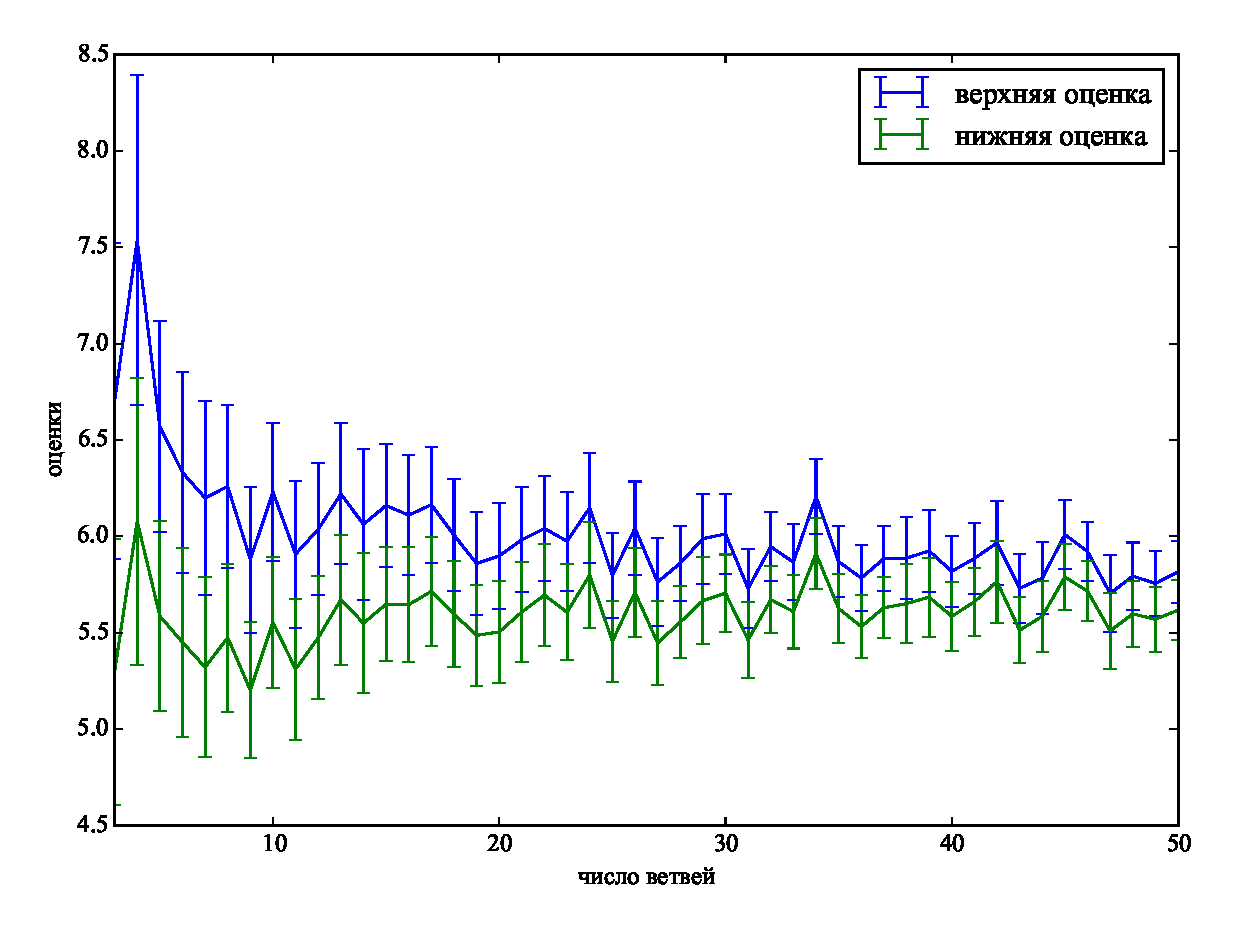
\includegraphics[width=0.8\textwidth]{convergence_to_true_value_standard}
	\caption{Верхняя и нижняя оценки стоимости опциона по алгоритму Броади-Глассермана.}
	\label{fig:true_value_test_standard}
	\footnotesize{Оценки стоимости опциона с начальной ценой 100 и ценой страйк 100, выписанного на срок 1 год на базовый актив с риск-нейтральной процентной ставкой $r = 0.05$, дивидендной ставкой $\delta = 0.1$ и волатильностью $\sigma=0.2$, цена которого --- случайный процесс, являющийся геометрическим броуновским движением с параметрами $\mu = r - \delta$ и $\sigma$, исполняемого 4 раза в году.}
\end{figure}
\begin{figure}[htpb]
    \centering
    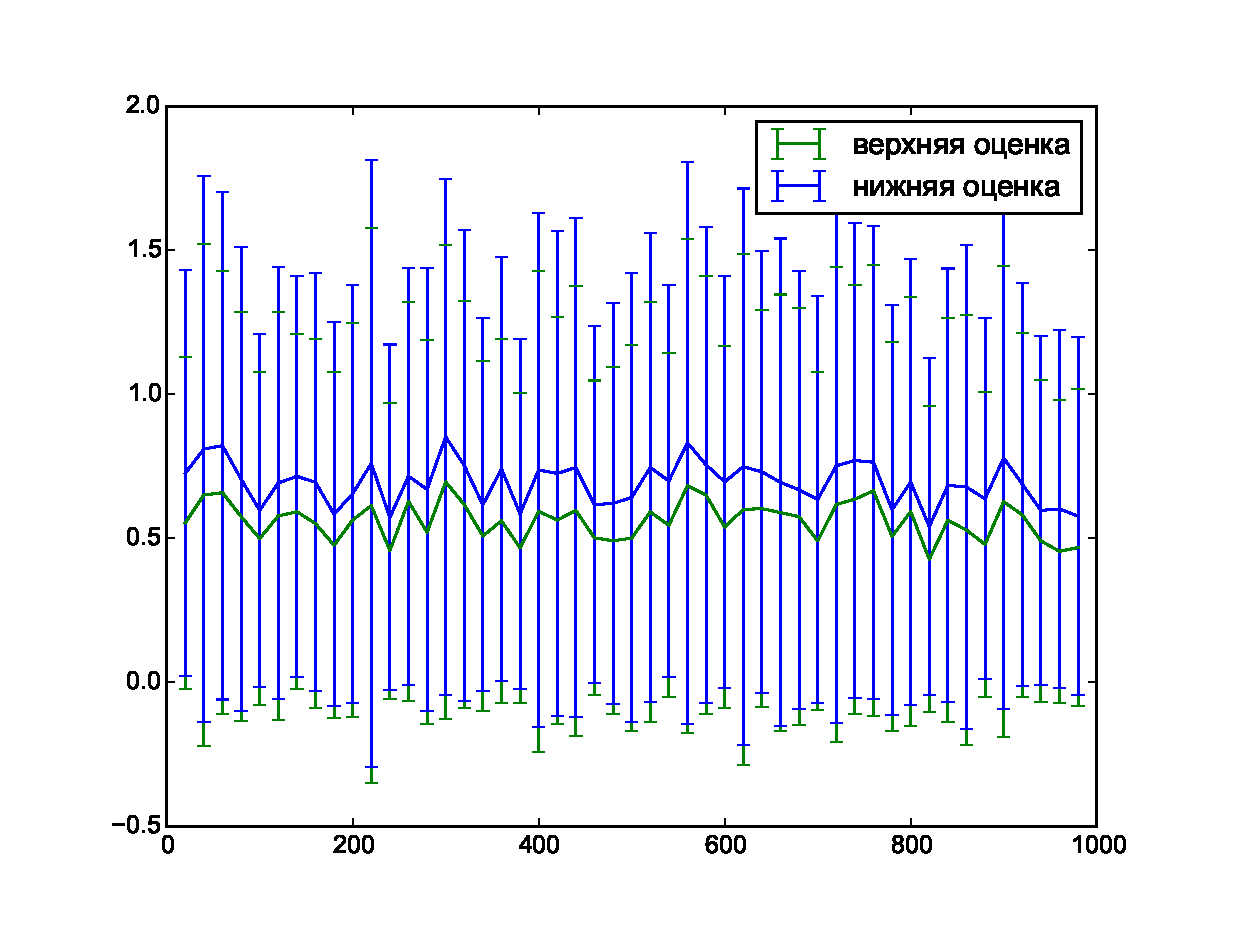
\includegraphics[width=0.8\textwidth]{convergence_to_true_value_random_subtree}
    \caption{Верхняя и нижняя оценки стоимости опциона по случайным поддеревьям.}
    \label{fig:random_subtree_modified_ev}
    \footnotesize{Оценки стоимости опциона с начальной ценой 100 и ценой страйк 100, выписанного на срок 1 год на базовый актив с риск-нейтральной процентной ставкой $r = 0.05$, дивидендной ставкой $\delta = 0.1$ и волатильностью $\sigma=0.2$, цена которого --- случайный процесс, являющийся геометрическим броуновским движением с параметрами $\mu = r - \delta$ и $\sigma$, исполняемого 4 раза в году.}
\end{figure}

Представление о порядке улучшения, обеспечиваемом обходом случайных поддеревьев, можно получить, изучив графики \ref{fig:rmse_over_nop_upper} и \ref{fig:rmse_over_nop_lower} . На первом из них представлено среднее отклонение от истинного значения для верхней оценки стоимости опциона различными методами: стандартным и усовершенствованным с изменением математического ожидания числа вершин, которые будут поглощены на $k$-м шаге, по линейному ($g_k = \nicefrac{k}{m}$), квадратичному ($g_k = \left(\nicefrac{k}{m}\right)^2$) и обратному квадратичному закону ($g_k = \sqrt{\nicefrac{k}{m}}$). Здесь видно, что средняя ошибка оценок относительно истинного значения цены опциона, полученных за одно и то же вычислительное время (число элементарных операций), для различных методов различаются слабо. 
\begin{figure}[HtPb]
    \centering
	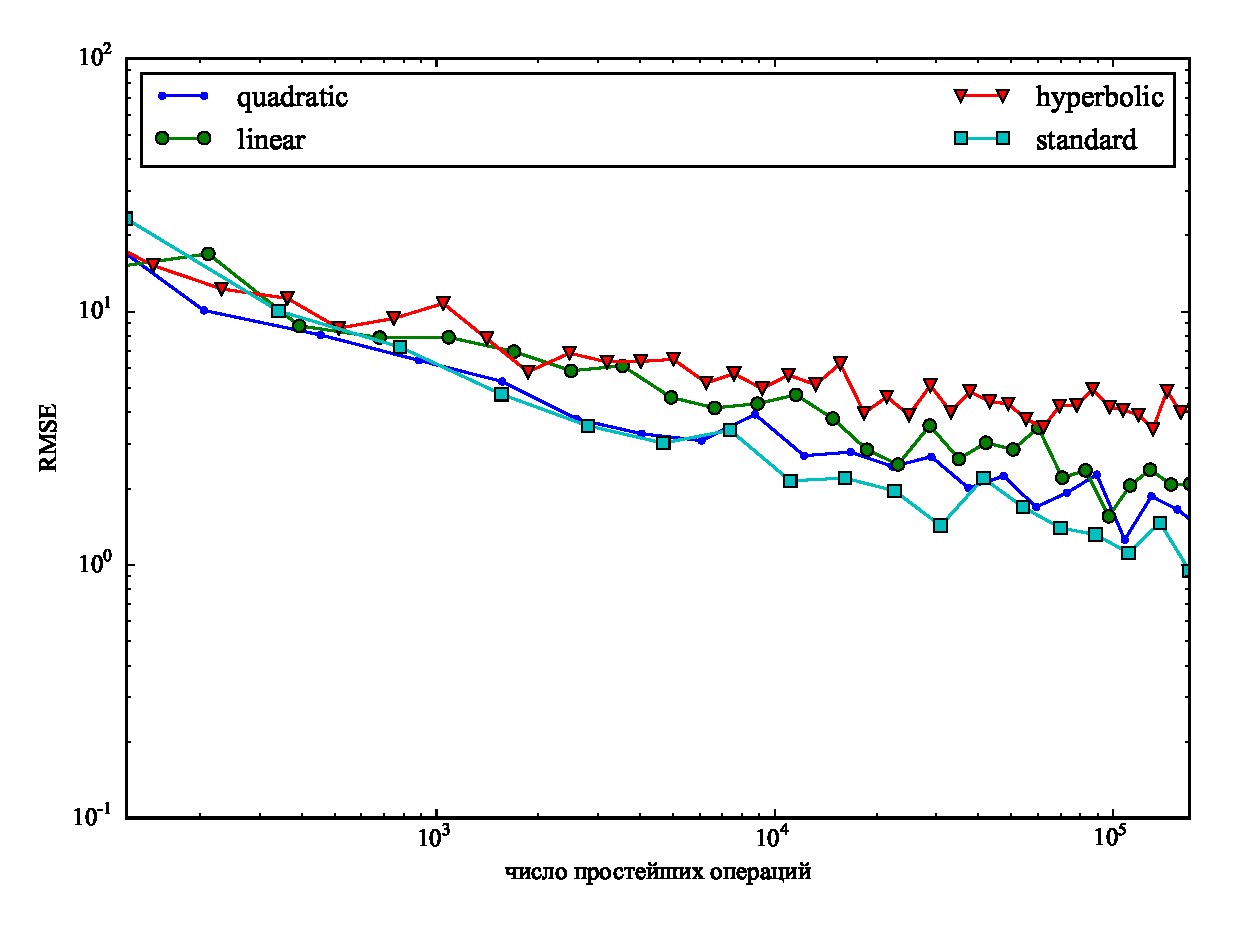
\includegraphics[width=0.8\textwidth]{rmse_over_nop_upper}
	\caption{Отклонение оценок стоимости опциона по полному дереву от истинного значения.}
	\label{fig:rmse_over_nop_upper}
	\footnotesize{Оценивается опцион с начальной ценой 100 и ценой страйк 100, выписанный на срок 1 год на базовый актив с риск-нейтральной процентной ставкой $r = 0.05$, дивидендной ставкой $\delta = 0.1$ и волатильностью $\sigma=0.2$, цена которого --- случайный процесс, являющийся геометрическим броуновским движением с параметрами $\mu = r - \delta$ и $\sigma$, исполняемый 6 раз в году.}
\end{figure}
\begin{figure}[HtPb]
    \centering
	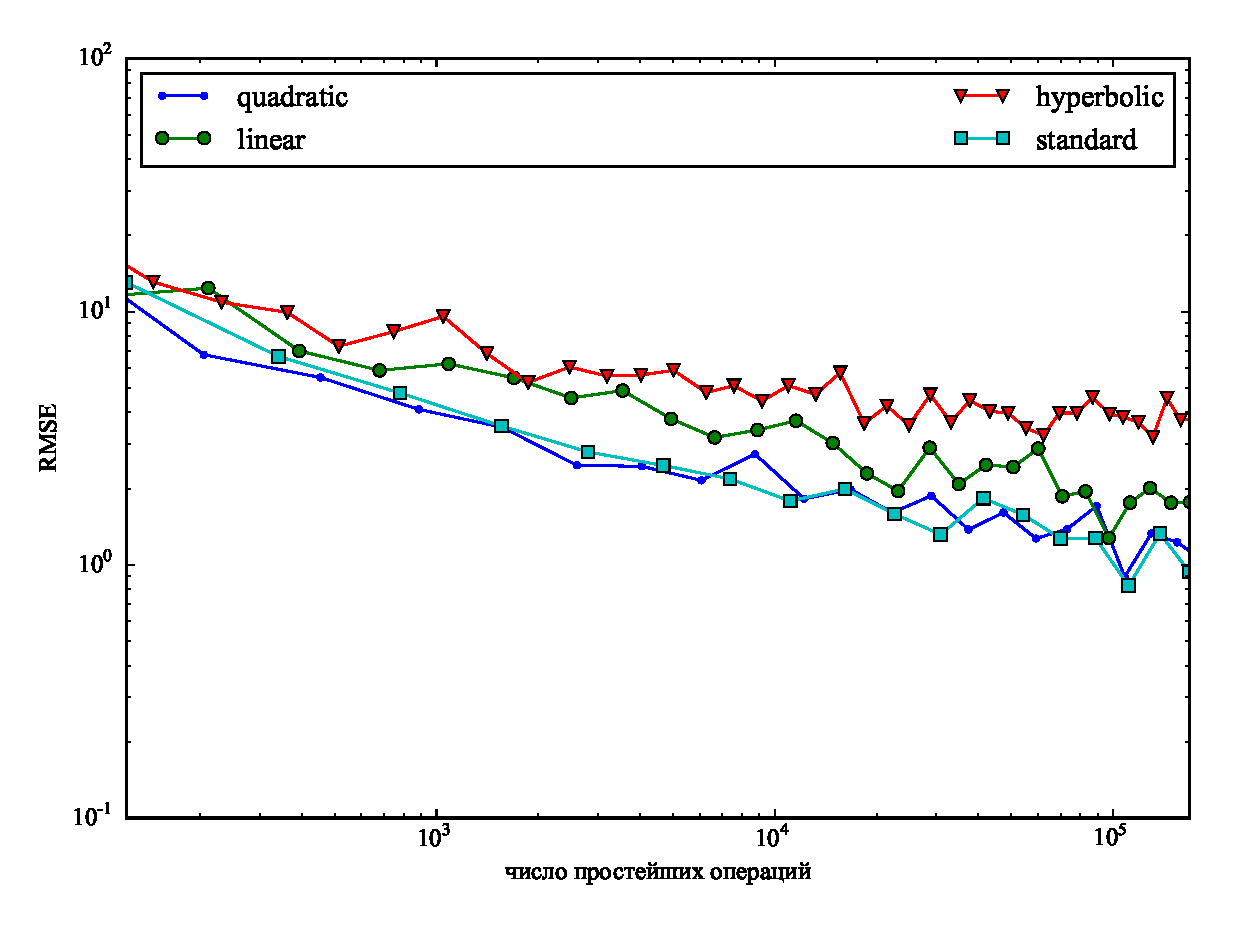
\includegraphics[width=0.8\textwidth]{rmse_over_nop_lower}
	\caption{Отклонение оценок стоимости опциона по случайным поддеревьям от истинного значения.}
	\label{fig:rmse_over_nop_lower}
	\footnotesize{Оценивается опцион с начальной ценой 100 и ценой страйк 100, выписанный на срок 1 год на базовый актив с риск-нейтральной процентной ставкой $r = 0.05$, дивидендной ставкой $\delta = 0.1$ и волатильностью $\sigma=0.2$, цена которого --- случайный процесс, являющийся геометрическим броуновским движением с параметрами $\mu = r - \delta$ и $\sigma$, исполняемый 6 раз в году.}
\end{figure}
